\documentclass[12pt,a4paper]{report}

\usepackage[T1]{fontenc}
\usepackage[utf8]{inputenc}
\usepackage[serbian,english]{babel}
\usepackage{geometry}
\usepackage{setspace}
\usepackage{amsmath}
\usepackage{graphicx}
\usepackage{float}
\usepackage{booktabs}
\usepackage{array}
\usepackage{caption}
\usepackage{subcaption}
\usepackage{hyperref}
\usepackage{xcolor}
\usepackage{titlesec}
\usepackage{fancyhdr}
\usepackage{enumitem}
\usepackage{longtable}

\geometry{
  left=30mm,
  right=25mm,
  top=25mm,
  bottom=25mm
}
\setlength{\headheight}{15pt}

\onehalfspacing
\setlength{\parindent}{1.25cm}
\setlength{\parskip}{0.35em}
\graphicspath{{../output/predictions/}{assets/}{assets/book_pages/}}

\hypersetup{
  colorlinks=true,
  linkcolor=black,
  urlcolor=blue,
  citecolor=black,
  pdftitle={Vizuelna procena kvaliteta hoda},
  pdfauthor={Student}
}

\pagestyle{fancy}
\fancyhf{}
\fancyhead[L]{Vizuelna procena kvaliteta hoda}
\fancyhead[R]{Ra\v{c}unarski vid}
\fancyfoot[C]{\thepage}

\titleformat{\chapter}[display]
  {\bfseries\Large}
  {\filcenter\chaptertitlename\ \thechapter}
  {0.5ex}
  {\filcenter}

\begin{document}
\selectlanguage{serbian}
\hypersetup{pageanchor=false}

\begin{titlepage}
  \thispagestyle{empty}
  \centering

  \begin{minipage}{0.21\textwidth}
    \centering
    
\includegraphics[width=\textwidth]{etf_logo.png}
  \end{minipage}
  \hfill
  \begin{minipage}{0.21\textwidth}
    \centering
    
\includegraphics[width=\textwidth]{etf_logo2.png}
  \end{minipage}

  \vspace{1.2cm}

  {\Large Univerzitet u Beogradu\par}
  \vspace{0.15cm}
  {\Large Elektrotehni\v{c}ki fakultet\par}
  \vspace{0.15cm}
  {\large Katedra za Signale i sisteme\par}

  \vspace{2.3cm}

  \vspace{2.4cm}

  {\Huge\bfseries Vizuelna procena kvaliteta hoda iz RGB videa\par}
  \vspace{0.45cm}
  {\Large Klasican pristup zasnovan na opti\v{c}kom toku, PCA modelu kretanja i regresiji\par}

  \vspace{2.1cm}

  \begin{tabular}{>{\bfseries}p{4.3cm}p{7.6cm}}
    Student: & Aleksa Mojsi\'{c} \\
    Broj indeksa: & 25/3319 \\
    Predmet: & Kompjuterska Vizija \\
  \end{tabular}

  \vfill

  {\large Beograd, avgust 2026.\par}
\end{titlepage}

\pagenumbering{roman}
\hypersetup{pageanchor=true}
\tableofcontents
\clearpage

\chapter*{Sa\v{z}etak}
\addcontentsline{toc}{chapter}{Sa\v{z}etak}
Ovaj rad razmatra problem vizuelne procene kvaliteta hoda humanoidnog agenta na
osnovu spoljnog RGB videa. Cilj projekta nije biomehani\v{c}ka analiza u
klini\v{c}kom smislu, ve\'{c} izgradnja reproduktivnog i interpretabilnog
pipeline-a koji iz video sekvence izvla\v{c}i gust opti\v{c}ki tok, formira
niskodimenzioni model kretanja i na kraju predvi\dj a ukupni skor i direktno
podr\v{z}ane ciljeve. Implementacija je zasnovana na klasi\v{c}nim metodama
ra\v{c}unarskog vida: preprocessing-u slike, translacionom poravnanju, gustim
poljima kretanja, PCA/SVD aproksimaciji i Ridge regresiji.

U radu se koristi skup od 56 bo\v{c}no renderovanih MuJoCo video sekvenci sa
vi\v{s}e scenarija kretanja. Pored numeri\v{c}kog skora, sistem generi\v{s}e
vizualizaciju opti\v{c}kog toka i heatmap temporalne energije kretanja. Eksperimentalni
rezultati pokazuju da kompletan sistem radi end-to-end, ali i da su trenutne
metrike za ukupni skor i stabilnost slabe. Zbog toga se projekat najbolje
posmatra kao funkcionalan prototip i dobra osnova za dalja unapredjenja, a ne
kao zavr\v{s}en sistem visoke ta\v{c}nosti.

\clearpage
\pagenumbering{arabic}

\chapter{Uvod}
Procena kvaliteta pokreta iz video sekvence predstavlja klasi\v{c}an problem na
preseku ra\v{c}unarskog vida, analize kretanja i procene kvaliteta akcije
(Action Quality Assessment). U op\v{s}tem slu\v{c}aju, zadatak podrazumeva da se
na osnovu same posmatrane sekvence proceni koliko je neko izvodjenje pokreta
stabilno, pravilno, ritmi\v{c}no i uskladjeno sa o\v{c}ekivanim obrascem.
Takav problem je naro\v{c}ito zanimljiv kada dodatne informacije nisu dostupne,
odnosno kada sistem ne vidi ni kontakte, ni sile, ni unutra\v{s}nja stanja
kontrolera, ve\'{c} isklju\v{c}ivo video snimak.

U ovom projektu fokus nije na ljudskom hodu iz klini\v{c}kih baza podataka, ve\'{c}
na humanoidnom agentu koji hoda u simulatoru i \v{c}iji se izlazi renderuju u
RGB video formatu. Ta postavka je korisna iz dva razloga. Prvo, omogu\'{c}ava
da se za svaki klip dobije izveden ciljni skor iz simulator telemetry signala.
Drugo, uvodi stroga ograni\v{c}enja u inferenciji: model za procenu kvaliteta
hoda koristi isklju\v{c}ivo video, bez direktnog pristupa internim podacima koji
su kori\v{s}\'{c}eni za formiranje target-a.

Polazna hipoteza rada glasi da se u vizuelnom obrascu hoda nalazi dovoljno
informacije za aproksimaciju ukupnog skora kvaliteta i nekoliko njegovih
komponenti. Ako je to ta\v{c}no, tada bi klasi\v{c}ni alati ra\v{c}unarskog vida
mogli da poslu\v{z}e kao transparentna alternativa te\v{s}kim dubokim modelima,
ili barem kao stabilan i interpretabilan baseline. U skladu sa tim, sistem je
namerno gra\dj en kao niz jasnih koraka: priprema frejmova, opti\v{c}ki tok,
poravnanje, PCA motion basis, temporalne osobine i regresija.

Va\v{z}no je naglasiti da ovde cilj nije da se simulacioni skor predstavi kao
medicinska istina. Naprotiv, skor je izvedena veli\v{c}ina konstruisana iz
simulatorskih signala. Time se dobijaju dosledne labele za eksperiment, ali se
istovremeno uvodi i osnovno ograni\v{c}enje rada: kvalitet target-a direktno
uti\v{c}e na kvalitet modela. Zbog toga se rezultati u ovom radu tuma\v{c}e
pre svega kao ocena funkcionalnosti pipeline-a i njegove sposobnosti da iz
vizuelnog signala izvu\v{c}e korisne indikatore kvaliteta hoda.

\chapter{Teorijska osnova}
Najve\'{c}i deo teorijskog oslonca za ovaj projekat dolazi iz knjige Richarda
Szeliskog \textit{Computer Vision: Algorithms and Applications}. Iako rad ne
implementira jedan gotov algoritam iz knjige u celini, gotovo svaka klju\v{c}na
faza sistema ima jaku vezu sa odgovaraju\'{c}im poglavljem: filtriranje i
preprocessing slike, procena kretanja, poravnanje, linearni podprostori i
least-squares modeli.

Prva va\v{z}na teorijska komponenta je gust opti\v{c}ki tok. U kontekstu ovog
projekta, opti\v{c}ki tok predstavlja procenu lokalnih pomeraja izmedju susednih
frejmova video sekvence. Na taj na\v{c}in se dinami\v{c}ka informacija iz hoda
pretvara u polje vektora koje direktnije opisuje kretanje tela nego same RGB
vrednosti. Ovaj izbor je prirodan, jer je kvalitet hoda mnogo vi\v{s}e povezan sa
ritmom, stabilno\v{s}\'{c}u i koordinacijom pokreta nego sa teksturom slike.

Druga komponenta je translaciono poravnanje. Ako kamera ili ceo agent imaju
izra\v{z}eno globalno kretanje kroz kadar, apsolutni opti\v{c}ki tok mo\v{z}e biti
dominiran tom velikom translacijom, pa sitnije razlike izmedju stabilnog i
nestabilnog hoda postaju te\v{z}e uo\v{c}ljive. Zbog toga se procenjuje
body-centered residual flow, odnosno tok iz koga je uklonjeno dominantno
globalno pomeranje. Takav signal je pogodniji za analizu obrasca samog hoda.

Tre\'{c}a komponenta je ideja nau\v{c}enih modela kretanja. Umesto da se svako
polje toka posmatra izolovano, vi\v{s}e uzastopnih polja se sla\v{z}e u visoku
dimenziju, centriraju se i dekomponuju preko SVD/PCA. Rezultat su bazna polja
kretanja i temporalni koeficijenti koji daju kompaktnu reprezentaciju
sekvence. Ta reprezentacija je interpretabilnija i mnogo pogodnija za jednostavniji
regresioni model od direktnog rada nad sirovim pikselima.

\begin{figure}[H]
  \centering
  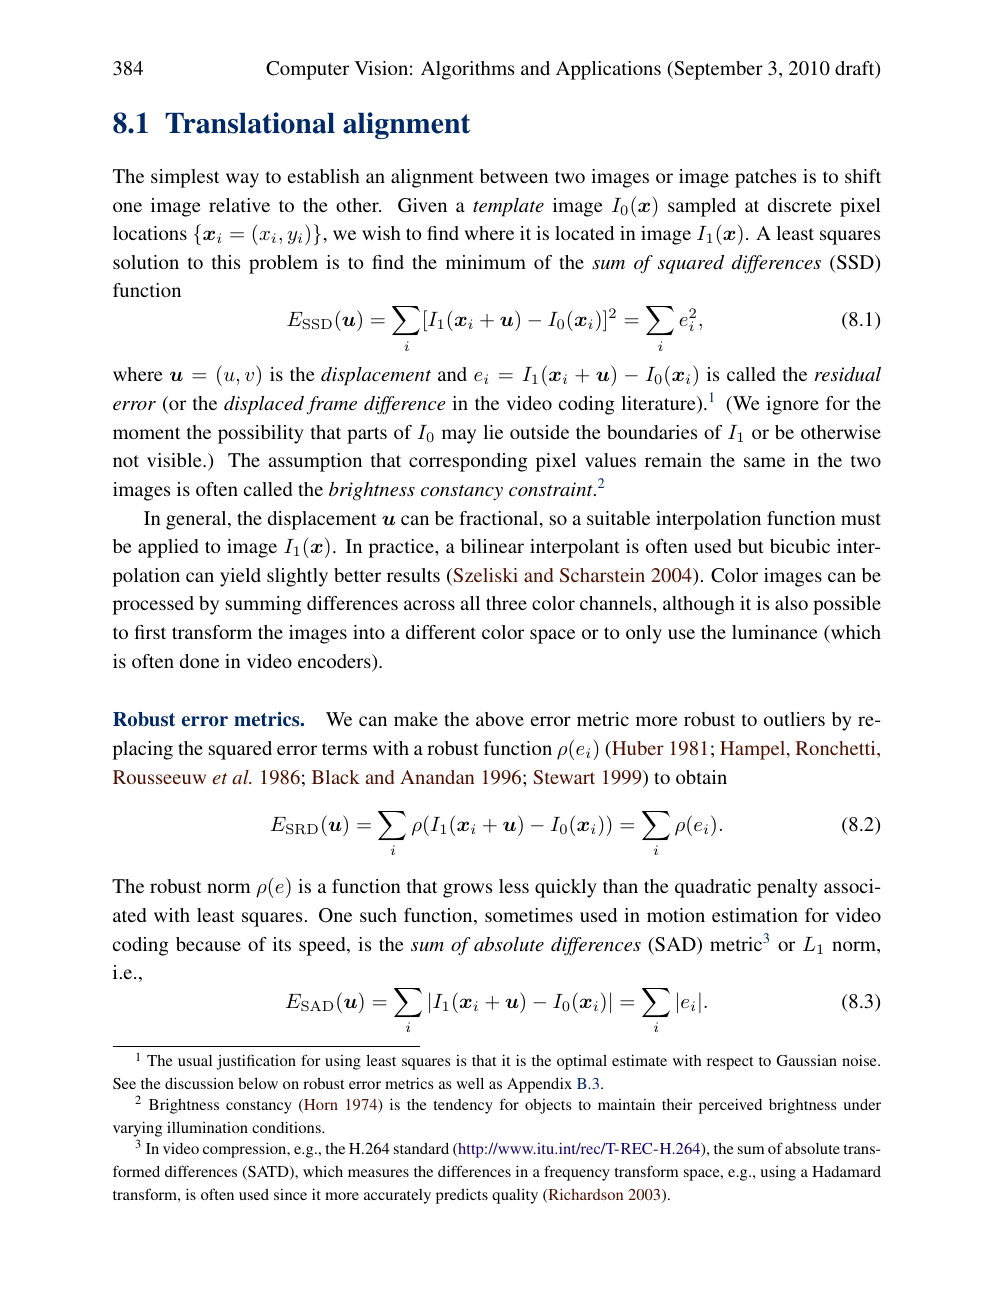
\includegraphics[width=0.86\textwidth]{szeliski_alignment-406.png}
  \caption{Strana iz Szeliski draft-a koja slu\v{z}i kao teorijska osnova za
  translaciono poravnanje i odvajanje globalnog i lokalnog kretanja
  (PDF strana 406).}
\end{figure}

\begin{figure}[H]
  \centering
  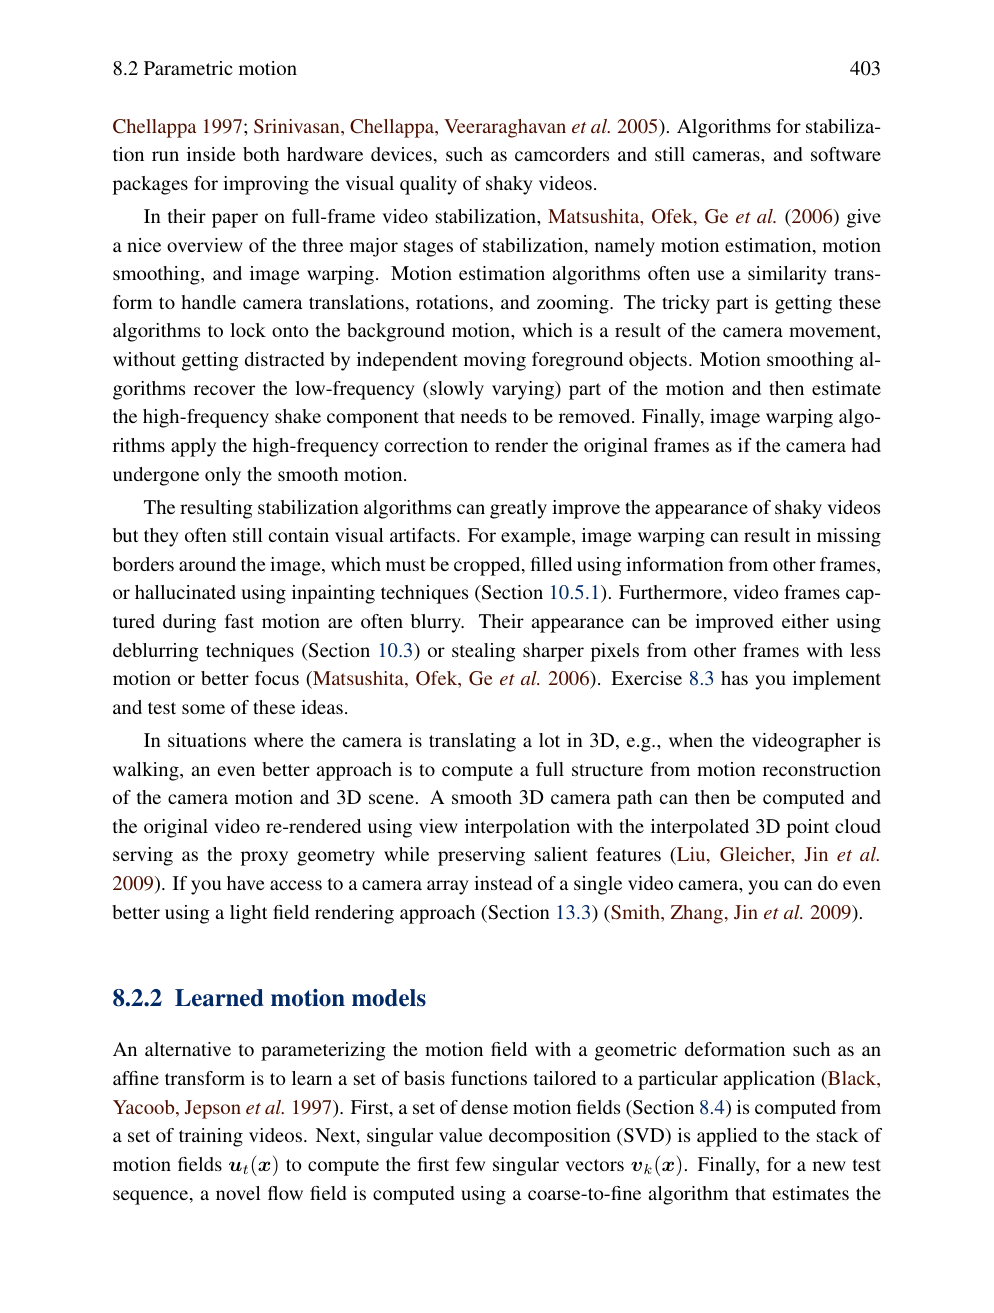
\includegraphics[width=0.86\textwidth]{szeliski_motion_basis-425.png}
  \caption{Strana iz Szeliski draft-a na kojoj se oslanja ideja nau\v{c}enih
  modela kretanja i PCA baznih vektora (PDF strana 425).}
\end{figure}

\begin{figure}[H]
  \centering
  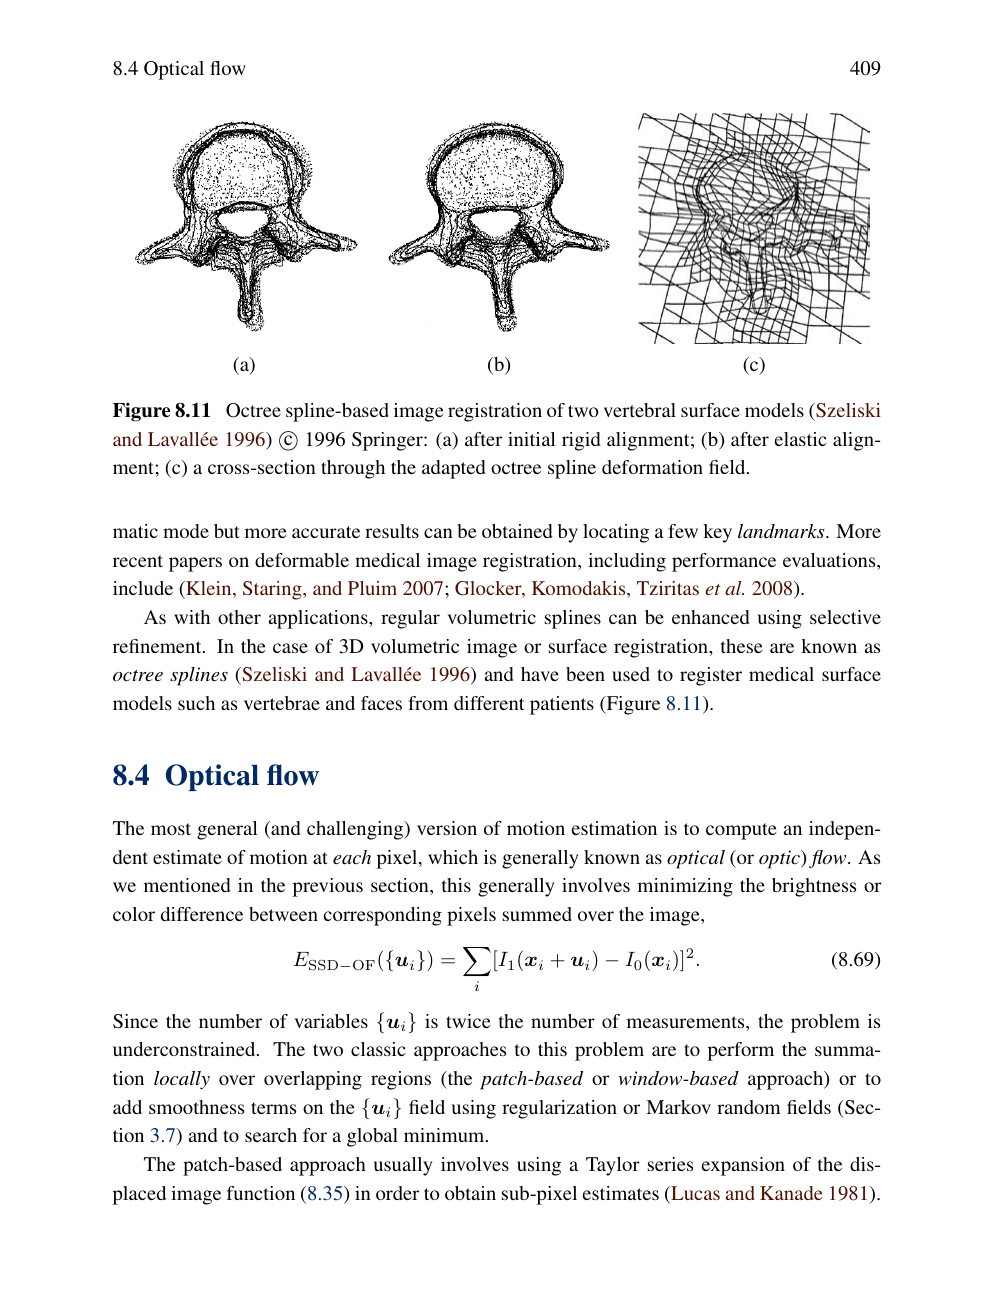
\includegraphics[width=0.86\textwidth]{szeliski_optical_flow-431.png}
  \caption{Strana iz Szeliski draft-a relevantna za gust opti\v{c}ki tok i
  formulaciju problema procene pomeraja izmedju frejmova (PDF strana 431).}
\end{figure}

Pored procene toka, bitna je i vremenska struktura hoda. Stabilan hod je
pribli\v{z}no periodi\v{c}an: koraci se smenjuju pravilnim ritmom, leva i desna
strana imaju o\v{c}ekivanu simetriju, a promene brzine nisu nasilne i nasumi\v{c}ne.
Zato su u projektu kori\v{s}\'{c}ene temporalne osobine zasnovane na autokorelaciji,
Furijeovim sa\v{z}ecima i promeni PCA koeficijenata kroz vreme. Na kraju, sve te
osobine ulaze u jednostavan ali stabilan regresioni model koji predvidja
ukupni skor i komponente kvaliteta hoda.

\chapter{Pregled implementacije}
Implementacija projekta je organizovana tako da prati prirodan tok obrade
video podataka. Modul \path{src/gait_aqa/data/} zadu\v{z}en je za pripremu
manifesta, rad sa ulaznim video klipovima i organizaciju dataset-a. Modul
\path{src/gait_aqa/vision/} predstavlja jezgro klasi\v{c}nog computer vision
pristupa: preprocessing frejmova, foreground obradu, procenu opti\v{c}kog toka,
poravnanje i izgradnju motion basis modela.

Posebni moduli sadr\v{z}e regresioni model, trening, evaluaciju metrika i
generisanje vizuelnih izlaza. Takva podela odvaja numeri\v{c}ku obradu od
prezentacije rezultata i \v{c}ini sistem lak\v{s}im za proveru.

U prakti\v{c}nom smislu, projekat se koristi kroz jedinstveni \texttt{gait-aqa}
CLI. Time se izbegavaju duplicirane wrapper skripte, a priprema podataka,
trening, evaluacija i scoring ostaju jasno odvojene podkomande.

\begin{table}[H]
  \centering
  \caption{Glavni delovi repozitorijuma i njihova uloga}
  \footnotesize
  \begin{tabular}{p{5.3cm}p{7.6cm}}
    \toprule
    Putanja & Uloga u sistemu \\
    \midrule
    \texttt{MUJOCO\_videos/gait\_dataset/} & Realno renderovani side-view klipovi za trening i test. \\
    \texttt{CMU\_reference\_videos/} & BVH walking reference i MuJoCo renderi. \\
    \texttt{data/manifests/} & CSV manifesti i train/val/test podele. \\
    \texttt{src/gait\_aqa/vision/} & Preprocessing, opti\v{c}ki tok, poravnanje i motion basis. \\
    \texttt{src/gait\_aqa/training/} & Trening klasi\v{c}nog baseline modela. \\
    \texttt{reports/} & PDF izve\v{s}taj, modeli, logovi, predikcije, vizuelni izlazi i LaTeX fajlovi. \\
    \bottomrule
  \end{tabular}
\end{table}

\chapter{Definicija skora}
Ukupni skor je preuzet direktno iz walker export-a i preslikan iz opsega
$[0,1]$ u $[0,100]$. Izvorni walker ga defini\v{s}e kao scenario-relative
te\v{z}inski prosek stabilnosti, pra\'{c}enja, uspravnosti i glatko\'{c}e:

\begin{equation*}
\begin{aligned}
\text{composite} = {} & 0.40 \cdot \text{stability}
+ 0.30 \cdot \text{tracking} \\
& + 0.20 \cdot \text{upright}
+ 0.10 \cdot \text{smoothness}
\end{aligned}
\end{equation*}

Kompaktni video manifest ne sadr\v{z}i originalne normalizovane komponente niti
\texttt{mean\_action\_rate\_norm}, pa ih nije mogu\'{c}e korektno rekonstruisati.
Ponovna min-max normalizacija na manjem lokalnom skupu promenila bi definiciju
target-a. Zato se koristi samo direktno podr\v{z}an ukupni skor, survival-derived
stability i indikator pada.

\begin{table}[H]
  \centering
  \caption{Komponente skora i njihovo tuma\v{c}enje}
  \begin{tabular}{p{4.2cm}p{8.7cm}}
    \toprule
    Komponenta & Zna\v{c}enje \\
    \midrule
    Overall & Sto puta izvorni \texttt{composite\_score}. \\
    Stability & Sto puta udeo sekvence pre prvog pada. \\
    Fall & Reset, terminalni dogadjaj ili survival manji od jedan. \\
    Ostale komponente & Nedostupne u trenutnom export-u; ostaju prazne. \\
    \bottomrule
  \end{tabular}
\end{table}

Model fituje samo ciljeve za koje postoje stvarne oznake. Nedostupne komponente
i nepravilnosti ostaju prazne umesto da im se dodeli ve\v{s}ta\v{c}ka vrednost
nula ili sto. U trenutnom export-u dostupni su ukupni skor, survival-derived
stability skor i indikator pada.

\chapter{Podaci i metodologija}
Glavni eksperiment u ovoj verziji projekta ne koristi sinteticki demo dataset,
ve\'{c} stvarne renderovane video klipove iz foldera
\texttt{MUJOCO\_videos/gait\_dataset/}. Svaki klip u manifestu sadr\v{z}i putanju do videa,
identitet politike, checkpoint, scenario, seed i oznaku ugla kamere. Manifest
jasno razlikuje dostupne ciljeve od praznih, nedostupnih komponenti.

U dataset-u koji je kori\v{s}\'{c}en za trenutni rezultat nalazi se 56 side-view klipova.
Podela je izvedena grupisano, tako da klipovi iz istog checkpoint-a ne procure
u train i test u isto vreme. To je va\v{z}no, jer bi bez toga model lako mogao da
``prepozna'' porodicu skoro identi\v{c}nih sekvenci umesto da nau\v{c}i op\v{s}te
vizuelne osobine kvalitetnog hoda.

\begin{table}[H]
  \centering
  \caption{Pregled trenutno kori\v{s}\'{c}enog skupa}
  \begin{tabular}{lr}
    \toprule
    Stavka & Vrednost \\
    \midrule
    Ukupan broj klipova & 56 \\
    Train split & 40 \\
    Validation split & 8 \\
    Test split & 8 \\
    Side pogled & 56 \\
    Scenariji & forward, forward\_slow, turn, diagonal \\
    Trajanje jednog klipa & oko 5 sekundi \\
    FPS & 30 \\
    \bottomrule
  \end{tabular}
\end{table}

Sama metodologija eksperimenta sastoji se od nekoliko koraka. Najpre se iz
svakog videa u\v{c}itavaju frejmovi i prolaze kroz osnovni preprocessing. Zatim
se ra\v{c}una gust opti\v{c}ki tok i po potrebi uklanja dominantna translacija.
Nakon toga se polja toka redukuju preko PCA motion basis pristupa, iz koeficijenata
se grade temporalne osobine, a na kraju se trenira Ridge regresor.

\begin{enumerate}[leftmargin=1.4cm]
  \item U\v{c}itavanje manifesta i video klipova.
  \item Preprocessing frejmova i ra\v{c}unanje gustog opti\v{c}kog toka.
  \item Fitovanje PCA motion basis modela samo na train split-u.
  \item Gradnja feature vektora iz toka, koeficijenata i temporalnih sa\v{z}etaka.
  \item Trening nezavisnih regresionih glava samo za dostupne ciljeve.
  \item Evaluacija na test split-u kroz MAE, RMSE, $R^2$, Spearman i pairwise ranking accuracy.
\end{enumerate}

Ovaj tok je metodolo\v{s}ki uskladjen sa bele\v{s}kama iz dokumenta
\path{reports/assets/docs/methodology.md}: nema leakage-a, nema upotrebe
simulator state-a tokom inferencije, a sav fokus je na onome \v{s}to je vidljivo
iz samog videa. To je bitan kvalitet rada \v{c}ak i kada metrike jo\v{s} nisu
zadovoljavaju\'{c}e.

\chapter{Vizuelne osobine i motion representation}
Najve\'{c}a prednost ovog projekta je to \v{s}to ne tretira video samo kao crnu
kutiju. Umesto toga, gradi se medju-reprezentacija koja je ljudski razumljiva.
Opti\v{c}ki tok prikazuje gde i kako se telo kre\'{c}e kroz kadar; residual flow
odvaja op\v{s}ti translacioni drift od relativnog kretanja delova tela; a PCA
koeficijenti kondenzuju dominantne obrasce hoda u nekoliko brojeva po
sekvenci.

Takva reprezentacija je korisna i sa in\v{z}enjerske i sa prezentacione strane.
Sa in\v{z}enjerske strane, omogu\'{c}ava da se uo\v{c}i gde model eventualno gre\v{s}i.
Sa prezentacione strane, \v{c}ini rad mnogo obja\v{s}njivijim od pristupa u kome bi
postojao samo jedan duboki model i jedna izlazna brojka.

Na slici koja prikazuje opti\v{c}ki tok mo\v{z}e se videti intenzitet i smer
lokalnog pomeranja. Heatmap temporalne energije dopunjuje taj pogled bez
neopravdane tvrdnje da clip-level regresor daje frame-level dijagnozu.

\chapter{Eksperimenti i rezultati}
Repo trenutno podr\v{z}ava pripremu realnog manifesta, trening klasi\v{c}nog
baseline modela, evaluaciju nad test split-om i pojedina\v{c}no skoringovanje
jednog videa uz vizuelne izlaze. To je va\v{z}no jer pokazuje da sistem nije samo
fragment koda, nego kompletan eksperimentalni tok koji mo\v{z}e da se pokrene od
po\v{c}etka do kraja.

Najvažniji numeri\v{c}ki rezultat je, medjutim, prili\v{c}no trezan: model u
trenutnoj formi ne posti\v{z}e dobru ta\v{c}nost za ukupni skor. Metrike sa
poslednjeg pokretanja date su u Tabeli~\ref{tab:metrics}.

\begin{table}[H]
  \centering
  \caption{Metrike na test split-u iz poslednjeg pokretanja}
  \label{tab:metrics}
  \begin{tabular}{p{4cm}rrrrr}
    \toprule
    Target & MAE & RMSE & $R^2$ & Spearman & Ranking \\
    \midrule
    overall\_score & 4.16 & 5.84 & -1.23 & -0.39 & 0.33 \\
    stability\_score & 6.59 & 6.62 & 0.00 & 0.00 & 0.00 \\
    \bottomrule
  \end{tabular}
\end{table}

Rezultati pokazuju da su \texttt{overall\_score} i \texttt{stability\_score}
trenutno slabi. Negativan $R^2$ zna\v{c}i da model u tim ciljevima prakti\v{c}no
ne obja\v{s}njava varijansu bolje od vrlo prostog baseline-a. Spearman korelacija
za ukupni skor je takodje negativna, \v{s}to zna\v{c}i da poredak klipova po
kvalitetu nije dobro uhva\'{c}en.

Konstantni baseline koji uvek vra\'{c}a prosek train skupa ima test MAE 3.51 i
RMSE 5.17, odnosno bolji je od trenutnog vizuelnog modela (MAE skill $-0.18$).
Ridge regularizacija
je izabrana samo na validation skupu ($\alpha=1000$), gde je smanjila MAE na
2.82, ali taj dobitak se nije preneo na jedinu izdvojenu test politiku.

Stability target ima veoma malu varijansu u test grupi, pa $R^2$, Spearman i
ranking ne nose korisnu informaciju. Rezultat potvr\dj uje izvr\v{s}ivost
pipeline-a, ali ne i generalizaciju na nove politike.

Zbog toga ove rezultate ne treba predstavljati kao ``jak model'', nego kao
po\v{s}ten i funkcionalan prototip. To nije lo\v{s}a pozicija za seminarski rad:
sistem je kompletan, reproduktivan i interpretabilan, a ograni\v{c}enja su jasno
vidljiva i obrazlo\v{z}ena.

\chapter{Vizuelni prikazi iz sistema}
Jedan od razloga zbog kojih je ovaj pristup i dalje vredan, uprkos slabijim
overall metrikama, jeste to \v{s}to generi\v{s}e kvalitetne medjuartefakte za
analizu. U nastavku su prikazani konkretni izlazi iz programa nad jednim
realnim video klipom.

\begin{figure}[H]
  \centering
  \begin{subfigure}{0.48\textwidth}
    \centering
    
\includegraphics[width=\textwidth]{audit_score_flow.png}
    \caption{Vizuelizacija opti\v{c}kog toka}
  \end{subfigure}
  \hfill
  \begin{subfigure}{0.48\textwidth}
    \centering
    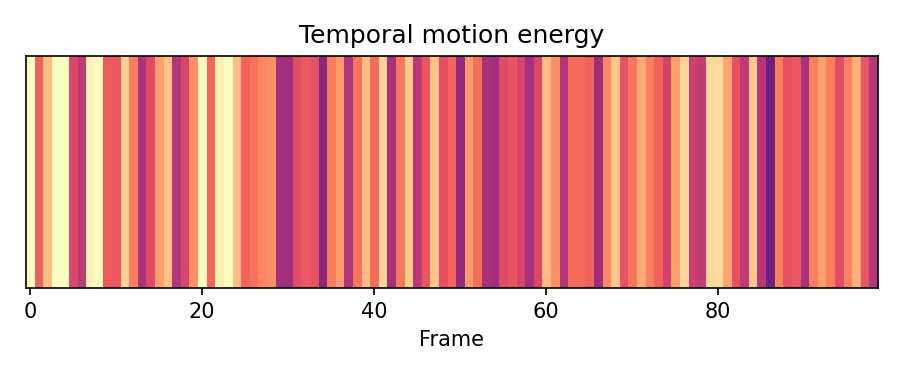
\includegraphics[width=\textwidth]{audit_score_motion_heatmap.png}
    \caption{Temporalna energija kretanja}
  \end{subfigure}
  \caption{Vizuelna obja\v{s}njenja koja generi\v{s}e sistem za jedan klip.}
\end{figure}

\begin{table}[H]
  \centering
  \caption{Primer procene po komponentama za jedan klip}
  \begin{tabular}{lr}
    \toprule
    Komponenta & Skor \\
    \midrule
    Overall & 57.18 \\
    Stability & 90.15 \\
    Fall probability & 0.98 \\
    Ostale komponente & nedostupne \\
    \bottomrule
  \end{tabular}
\end{table}

Ovi izlazi su korisni zato \v{s}to omogu\'{c}avaju dvostruko tuma\v{c}enje.
Sa jedne strane, korisnik dobija kona\v{c}an numeri\v{c}ki skor. Sa druge strane,
mo\v{z}e da vidi za\v{s}to je model do\v{s}ao do te procene i kako izgleda dinami\v{c}ki
obrazac na kojem se odluka zasniva. Upravo taj deo \v{c}ini rad mnogo
uverenljivijim od obi\v{c}nog CSV izlaza bez ikakvog vizuelnog konteksta.

\chapter{Diskusija}
Najpoštenije je re\'{c}i da rezultati potvr\dj uju dve stvari istovremeno.
Prva je da je vizuelni signal dovoljan da se iz njega izvuku smislene
karakteristike kretanja i napravi kompletan sistem za scoring. Druga je da taj
signal, u trenutnom obliku feature-a i target definicije, nije dovoljan da da
jak i stabilan model za ukupni kvalitet hoda.

Vi\v{s}e je mogu\'{c}ih razloga za to. Prvi je mali skup podataka: 56 klipova je
relativno malo za zadatak u kome postoji vi\v{s}e scenarija i seed-ova, ali samo
sedam nezavisnih politika. Drugi razlog je sama priroda target-a. Ukupni skor nije ru\v{c}no
ocenjivana ljudska oznaka, ve\'{c} simulaciono izvedena veli\v{c}ina koja mo\v{z}da ne
ima dovoljno direktan vizuelni ekvivalent u svakom trenutku sekvence.

Tre\'{c}i razlog je mali broj nezavisnih grupa: dva seed-a iste politike ne
predstavljaju dve nove politike. Aktivni eksperiment zato namerno koristi samo
kanonski side pogled, bez me\v{s}anja front-oblique snimaka.

Ipak, ovaj rad nije bez doprinosa. Naprotiv, kao studentski projekat on ve\'{c}
ispunjava nekoliko va\v{z}nih kriterijuma: postoji jasna ideja, direktna veza sa
literaturom, potpuno funkcionalna implementacija, eksperimentalni tok koji se
mo\v{z}e ponoviti i po\v{s}tena analiza ograni\v{c}enja. To je dobra osnova za slede\'{c}u
fazu rada, u kojoj bi se mogla uvesti analiza po uglovima kamere, ve\'{c}i skup
sekvenci ili duboki video baseline za poredjenje.

\chapter{Ograni\v{c}enja i budu\'{c}i rad}
Najva\v{z}nije ograni\v{c}enje rada jeste to \v{s}to ciljni skor poti\v{c}e iz simulatora,
a ne iz nezavisne ljudske ili klini\v{c}ke procene. Zbog toga model zapravo ne
u\v{c}i ``kvalitet hoda'' u op\v{s}tem smislu, ve\'{c} aproksimaciju jedne specifi\v{c}ne
definicije kvaliteta koju je nametnuo izvor podataka.

Drugo ograni\v{c}enje je \v{s}to RGB video ne nosi direktnu informaciju o kontaktima,
silama i unutra\v{s}njoj stabilnosti kontrolera. Neke nepravilnosti se mogu videti,
ali neke ostaju skrivene. To posebno poga\dj a komponente koje u sebi imaju ja\v{c}i
dinami\v{c}ki ili kontaktni karakter.

Tre\'{c}e ograni\v{c}enje je veli\v{c}ina i homogenost skupa. Iako postoji vi\v{s}e
scenarija, aktivni side-view dataset je i dalje relativno mali. Za bolju procenu
op\v{s}tosti modela bilo bi korisno imati vi\v{s}e klipova, vi\v{s}e politika i
odvojene eksperimente po kameri, scenariju i tipu hoda.

Najvažniji pravci budu\'{c}eg rada su:
\begin{itemize}
  \item unapredjenje target definicije i njene bolje veze sa vizuelno merljivim osobinama;
  \item ve\'{c}i skup realno renderovanih sekvenci;
  \item odvojena analiza po uglovima kamere i scenarijima;
  \item poredjenje sa \texttt{reference\_videos/} walking skupom;
  \item uvodjenje jednog modernog deep video baseline-a kao kontrasta klasi\v{c}nom pristupu.
\end{itemize}

\chapter{Zaklju\v{c}ak}
U radu je predstavljen kompletan pipeline za vizuelnu procenu kvaliteta hoda iz
RGB video sekvenci. Sistem koristi klasi\v{c}ne metode ra\v{c}unarskog vida,
inspirisane Szeliski literaturom, i kombinuje ih sa jednostavnim regresionim
modelom. Klju\v{c}na vrednost projekta nije u tome \v{s}to trenutno posti\v{z}e
izvanredne metrike, nego u tome \v{s}to je metodolo\v{s}ki jasan, reproduktivan i
interpretabilan.

Eksperimenti pokazuju da pipeline radi od manifesta do H.264 izlaza, ali da
ukupan skor ne generalizuje dobro na izdvojenu politiku. Zbog toga je najkorektnije re\'{c}i da je
projekat trenutno funkcionalan prototip sa jasnim potencijalom za dalje
unapredjenje.

Za studentski projekat to je i dalje dobar ishod: postoji ozbiljna veza izmedju
teorije i implementacije, pokazana je sposobnost da se izgradi i evaluira
kompletan sistem, a ograni\v{c}enja nisu sakrivena nego eksplicitno analizirana.
Upravo ta kombinacija tehni\v{c}ke realizacije i po\v{s}tene diskusije daje ovom
radu akademsku vrednost.

\chapter*{Literatura}
\addcontentsline{toc}{chapter}{Literatura}
\begin{enumerate}
  \item Richard Szeliski, \textit{Computer Vision: Algorithms and Applications},
  draft version, September 3, 2010.
  \item Gunnar Farneback, \textit{Two-Frame Motion Estimation Based on Polynomial Expansion}, 2003.
  \item PECoP: \textit{Parameter Efficient Continual Pretraining for Action Quality Assessment}, WACV 2024.
  \item CARE-PD repository, inspected as conceptual reference for AQA and rehabilitation scoring.
  \item Projekat \texttt{mujoco-bipedal-joystick-walker}, kori\v{s}\'{c}en kao izvor renderovanih sekvenci i label signala.
  \item Resty Wulanningrum, Anik Nur Handayani i Heru Wahyu Herwanto,
  \textit{DissabledGait: Gait Dataset of Normal People and People with
  Disabilities}, Mendeley Data, version 2, 2024,
  DOI: \texttt{10.17632/v6hy35ydch.2}.
  \item Edward Guillen Pinto, Leonardo Ramirez Lopez i Carlos Ramos Linares,
  \textit{GaHu-Video: Parametrization System for Human Gait Recognition},
  Mendeley Data, version 1, 2020, DOI: \texttt{10.17632/gprg4s73v4.1}.
  \item \textbf{Mogu\'{c}i dodatni skup podataka:} OU-ISIR Gait Database,
  Treadmill Dataset, Osaka University. Pristup zahteva potpisan institucionalni
  release agreement i posebno odobrenje; skup je zato evidentiran samo kao
  kandidat za budu\'{c}i rad.
\end{enumerate}

\end{document}
